
\section{Auswertung}
Die gemessenen Werte des Versuchs sind im Anhang als Kopie beigefügt.
\subsection{Magnetische Flussdichte zweier Spulen}
Im ersten Teil des Versuchs wird eine längere Spule betrachtet. Dabei wird die Flussdichte
im Verhältnis zum Abstand $x$ gemessen. Die Messwerte für diesen Teil der Messung sind im
Anhang zu finden. Mit Formel \ref{eqn:2} wird zuerst das Magnetfeld theoretisch berechnet.
Daraus folgt
\begin{align}
B\ua{theo} &= \SI{2.591}{\milli\tesla}\,.
\end{align}
\newline
\begin{figure}
  \centering
  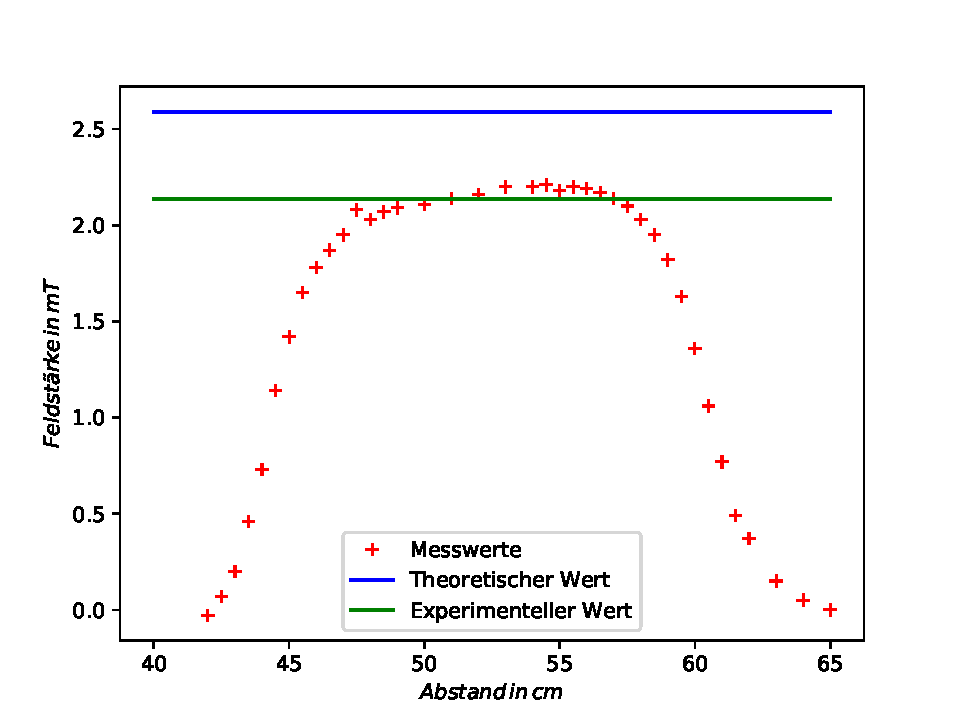
\includegraphics[width = 12 cm]{Spulelang2-2.pdf}
  \caption{Verhältnis der gemessenen Feldstärke zum Abstand für eine 16\,cm lange Spule}
  \label{fig:Messunga}
\end{figure}
Der experimentellen Wert des Magnetfelds wird mit
\begin{equation}
  \bar{x} = \frac{1}{n} \sum{x_n}
  \label{Mittelwert}
\end{equation}
berechnet. Für die Standardabweichung gilt
\begin{equation}
\upsigma = \frac{1}{\sqrt{n}} \sqrt{\frac{\sum{(x_n - \bar{x})^2}}{n-1} }.
\label{Standardabweichung}
\end{equation}
Daraus folgt
\begin{align}
B\ua{exp} &= \SI{2.136 \pm 0.031}{\milli\tesla}\,.
\end{align}

Im zweiten Teil des Versuchs werden die selben Messungen mit einer kürzeren Spule
durchgeführt. Daraus folgt
\begin{align}
B\ua{theo} &= \SI{2.286}{\milli\tesla}\,.
\end{align}
\begin{figure}
  \centering
  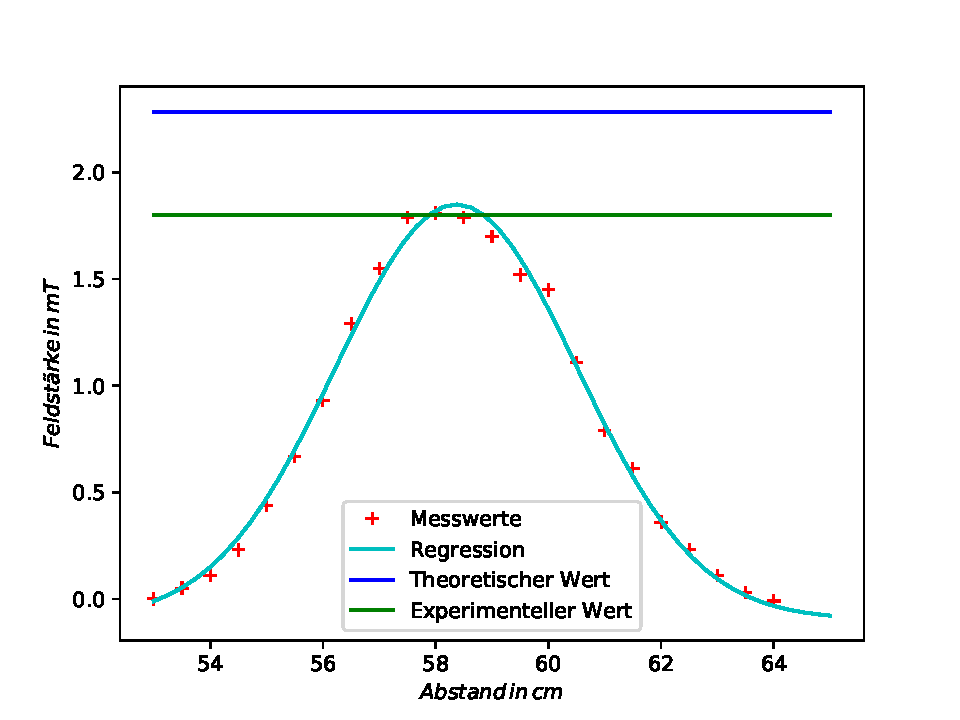
\includegraphics[width = 12 cm]{Spuleklein2-2.pdf}
  \caption{Verhältnis der gemessenen Feldstärke zum Abstand für eine 4\,cm lange Spule}
  \label{fig:Messunga}
\end{figure}
Mit Hilfe von Formel \eqref{Mittelwert} und \eqref{Standardabweichung} folgt
\begin{align}
B\ua{exp} &= \SI{1.773 \pm 0.025}{\milli\tesla}\,.
\end{align}
\newpage

\subsection{Helmholzspule}
Die magnetische Flussdichte eines Helmholzspulenpaar wird dreimal bestimmt.
Dabei werden Messungen innerhalb und außerhalb des Spulenpaars durchgefüht.
Dafür wird das Spulenpaar zu erst in einem Abstand von 8\,cm aufgestellt.

\begin{figure}
  \centering
  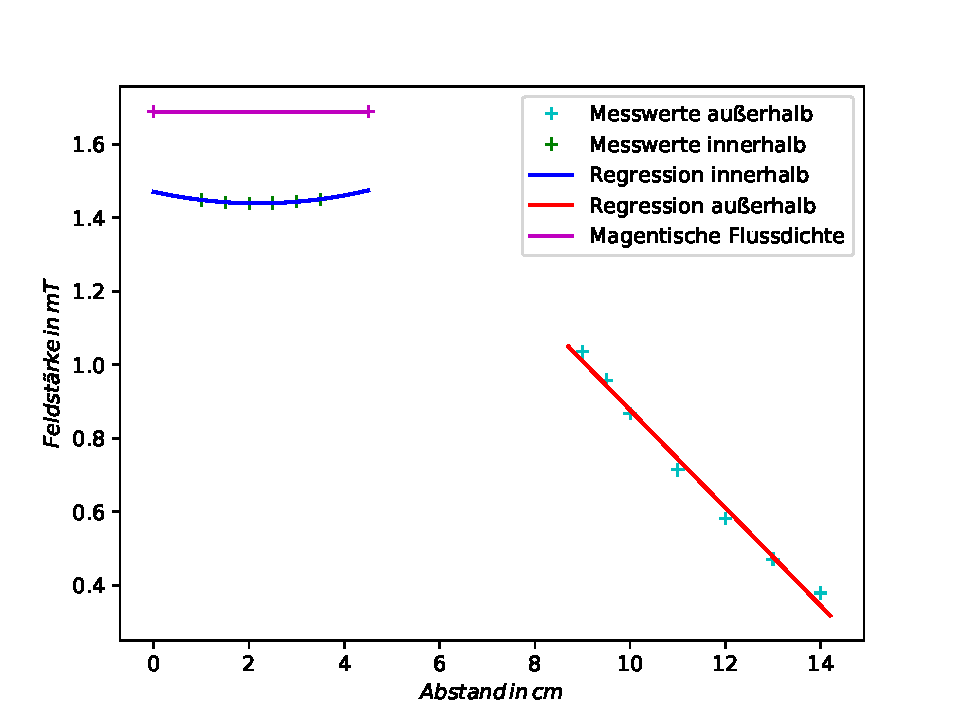
\includegraphics[width = 12 cm]{Helmholzspule8-2.pdf}
  \caption{Verhältnis der gemessenen Feldstärke zum Abstand für die Helmolzspule, 8\,cm}
  \label{fig:Messungb}
\end{figure}

%Für die magnetische Flussidichte des Helmholzspulenpaars ergibt sich mit Formel \ref

\begin{align}
B\ua{8cm} &= \SI{1.689}{\milli\tesla}\,.
\end{align}

\newpage
Für einen Abstand von 11\,cm ergibt sich für die magnetische Feldstärke
\begin{align}
B\ua{11cm} &= \SI{0.820}{\milli\tesla}\,.
\end{align}
\begin{figure}
  \centering
  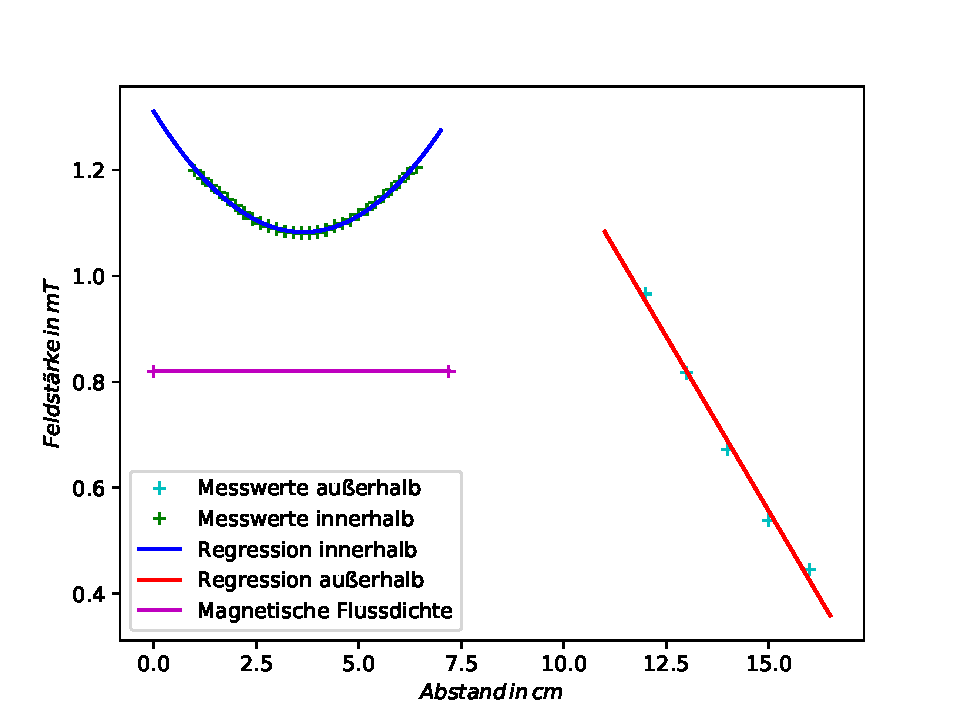
\includegraphics[width = 12 cm]{Helmholzspule11-2.pdf}
  \caption{Verhältnis der gemessenen Feldstärke zum Abstand für die Helmolzspule, 11\,cm}
  \label{fig:Messungb}
\end{figure}

\newpage
Im letzten Teil der Helmholzspule wird die magnetische Flussdichte im Abstand des
Spulenpaars von 14\,cm bestimmt. Daraus ergibt sich ein Wert von
\begin{align}
B\ua{14cm} &= \SI{0.490}{\milli\tesla}\,.
\end{align}
\begin{figure}
  \centering
  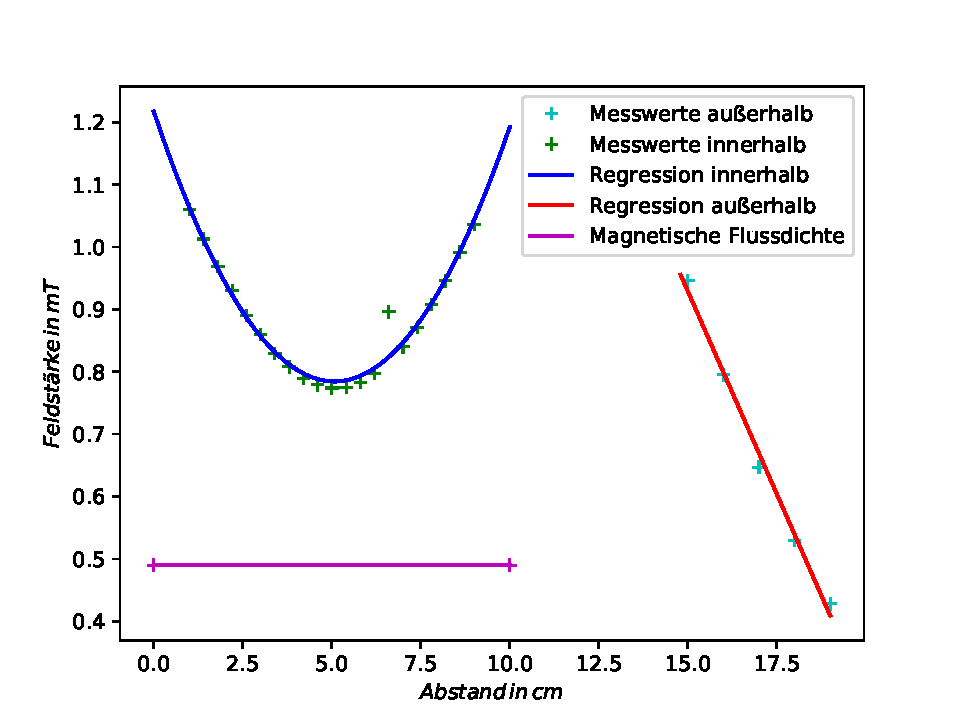
\includegraphics[width = 12 cm]{Helmholzspule14-2.pdf}
  \caption{Verhältnis der gemessenen Feldstärke zum Abstand für die Helmolzspule, 14\,cm}
  \label{fig:Messungb}
\end{figure}
\newpage

\subsection{Hysteresekurve}
Die in Abbildung (\ref{fig:hys}) zu sehende Hysteresekurve ensteht aus den gemessenen Werten,
die im Anhang zu finden sind.

  \begin{figure}
\centering
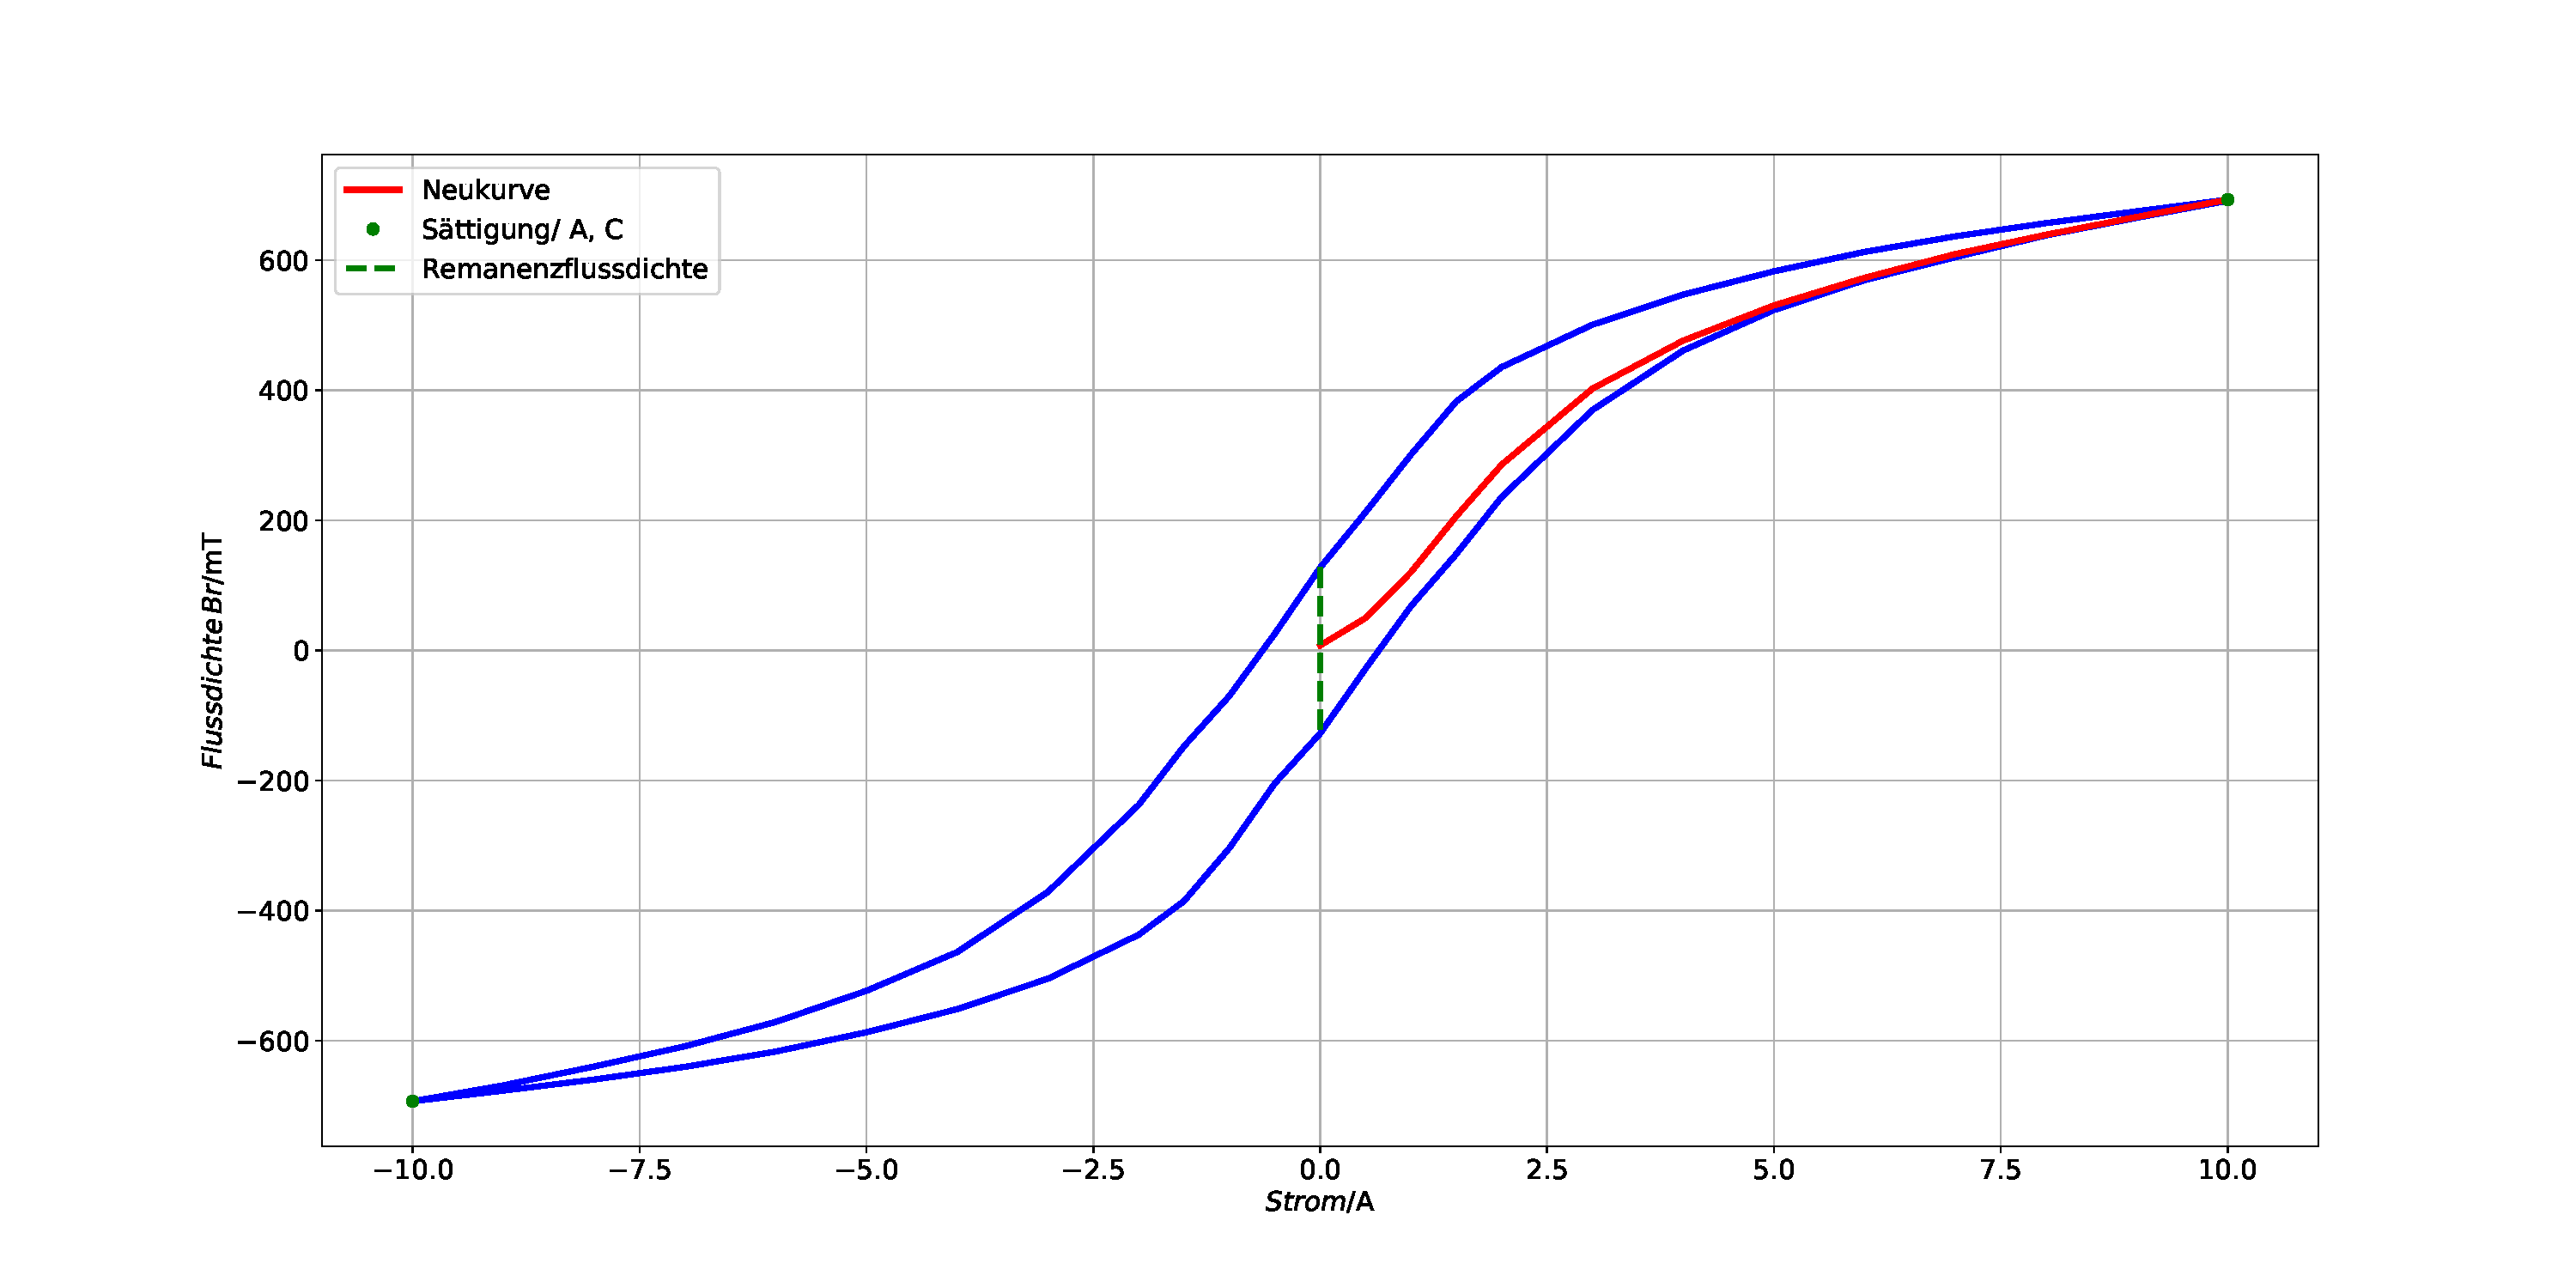
\includegraphics[width=\textwidth]{plothys.pdf}
\caption{Die Hysteresekurve}
\label{fig:hys}
\end{figure}
Die Neukurve führt zu Sättigungspunkt $A$ , der bei $692\, \mathrm{mT}$ liegt.
Nachdem kompletten Durchlauf liegt der Wert bei $691,3 \,\mathrm{mT}$.
Somit folgt:
\begin{equation*}
  A = (691,650 \pm 0,001)\, \mathrm{mT}
\end{equation*}
Der Sättigungspunkt $C$ wurde nur einmal durchlaufen.
Der Wert liegt bei
\begin{equation*}
  C = -693 \,\mathrm{mT}
\end{equation*}
 Die Remanenzflussdichte $B_r$ liegt bei
 \begin{align*}
   B_{r1} &= 127,4\, \mathrm{mT} & B_{r2} &= -127,5 \, \mathrm{mT}
 \end{align*}
 Für die Bestimmung der Koerzitivkraft wurde eine Ausgleichsrechnung mittels Python durchgeführt.
 Die Ausgleichsfunktion lautet:
 \begin{equation}
  f(x) = 693 \cdot \tanh(a\cdot(x + b)) + c
 \end{equation}
 Die Parameter für die Funktion von dem Weg von $A$ nach $C$ lautet:
 \begin{align*}
 a &= (0,247 \pm 0,006)\, \mathrm{\frac{1}{A}}\\
 b &= (0,74 \pm 0,07)\, \mathrm{A}\\
 c &= (-4 \pm 7)\, \mathrm{mT}
 \end{align*}

\begin{figure}
\centering
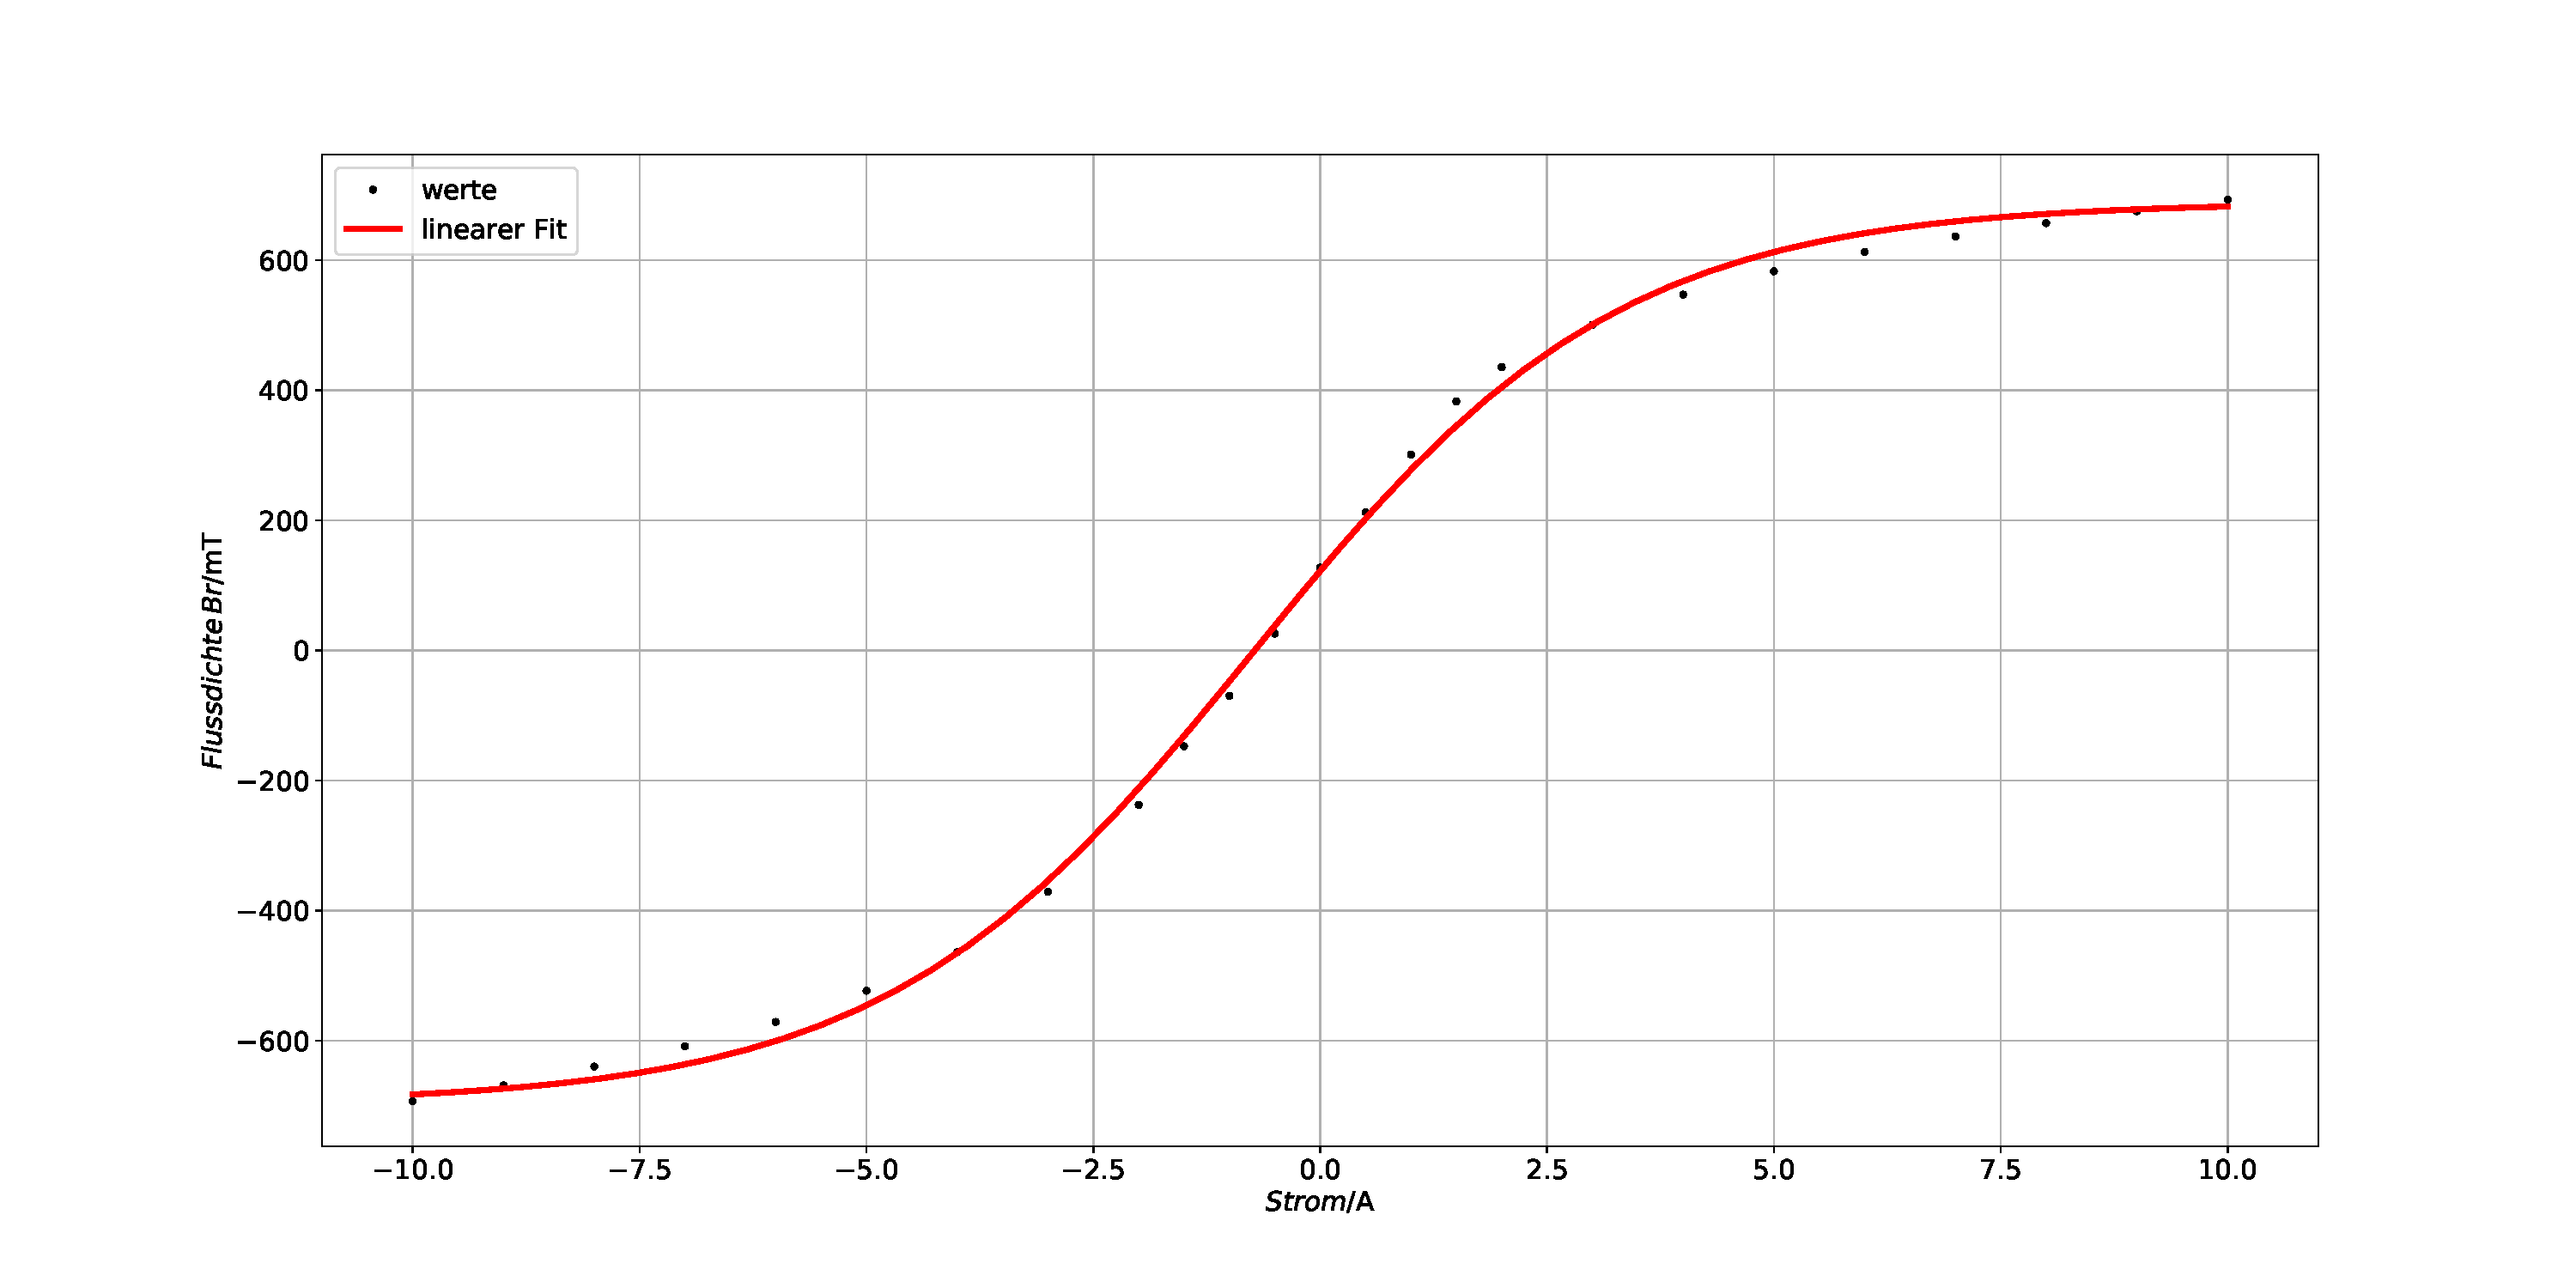
\includegraphics[width=\textwidth]{plotkoertiv.pdf}
\caption{Weg A - C}
\label{fig:koe}
\end{figure}

\begin{figure}
\centering
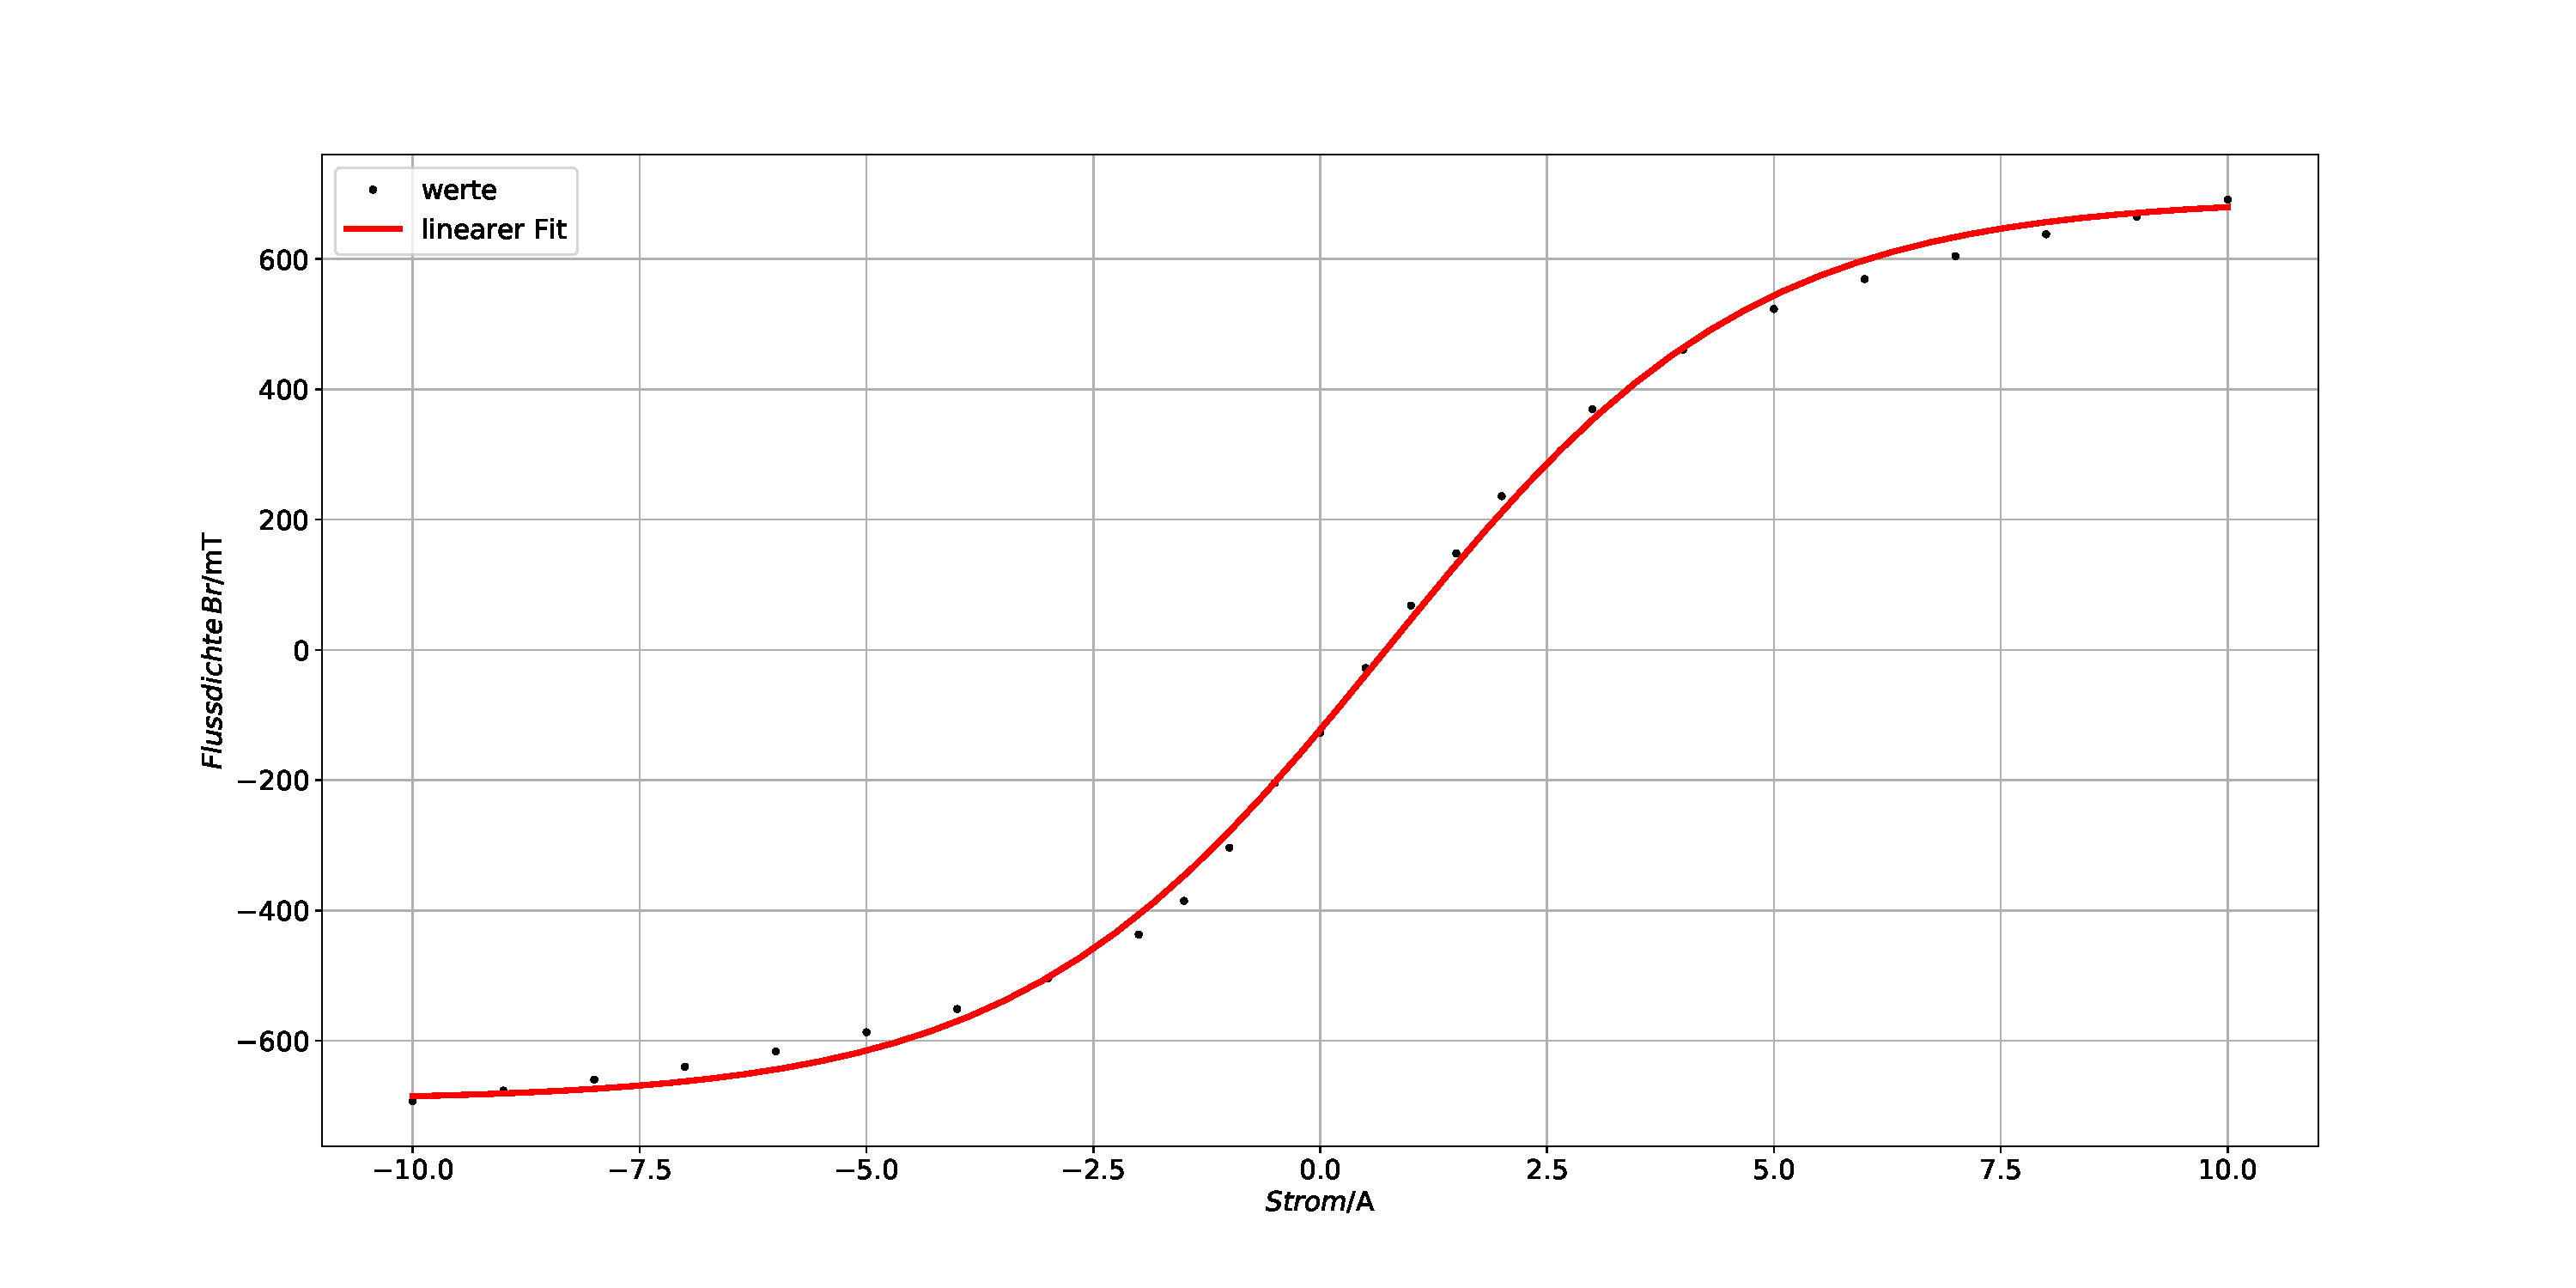
\includegraphics[width=\textwidth]{plotkoertiv2.pdf}
\caption{Weg C - A}
\label{fig:koe2}
\end{figure}
Die Parameter für den Weg von $C$ nach $A$ lauten:
 \begin{align*}
   a &= (0,247 \pm 0,005) \, \mathrm{\frac{1}{A}}\\
   b &= (-0,73 \pm 0,07)\, \mathrm{A} \\
   c &= (1 \pm 7) \, \mathrm{mT}\,
 \end{align*}
 Da die $b$-Werte die Verschiebung auf der x-Achse beschreiben, folgt daraus für die Koerzitivkraft $K$:
 \begin{equation*}
   K = (0,735 \pm  0,001) \, \mathrm{A}
\end{equation*}
\section{Diskussion}
Für die Bestimmung der magnetischen Flussdichten der einzelnen Spulen und des Helmholzspulenpaars
kam es beim Abnehmen der Messwerte zu einigen Ungenauigkeiten. In der folgenden Tabelle sind diese
noch einmal aufgelistet:
\begin{table}
  \centering
  \caption{Bestimmte Werte für die magnetische Flussdichte}
  \label{tab:Zusammenfassung}
  \begin{tabular}{c | c c c c}
    \toprule  $\text{Messung}$ & $3.1\ua{theo}$ & $3.1\ua{exp}$ & $3.2\ua{theo}$ & $3.2\ua{exp}$\\
    \midrule  $B$ & $2,591$ & $2,136$ &
              $2,286$ & $1,800$\\
    \bottomrule
  \end{tabular}
\end{table}

Wie in der Tabelle zu sehen ist, sind die Abweichungen von den gemessen Flussdichten zu den
theoretischen doch relativ groß. Besonders die Messapperaturen waren sehr anfällig für Berührungen. Zusätzlich war es schwierig mit Hilfe der Messonde die magnetische
Flussdichte genau in der Mitte der Spule zu messen.
\newline
Bei den drei Messungen mit dem Helmholzspulenpaar ist deutlich geworden, dass der ideale Abstand zwischen
beiden Spulen vorhanden ist, wenn der Radius der Spulen gleich ihrem Abstand ist. Ist dies der Fall überlagern sich
beide Einzelfelder und das Magnetfeld ist konstant. Mit zunehmenden Abstand wird die Überlagerung
der Einzelfelder immer geringer und die Einzelfelder sind viel deutlicher zu erkennen. Dies ist bei einem Abstand von
$11\, \text{cm}$ und $14\, \text{cm}$ deutlich zu sehen. Die magnetische Feldstärke nimmt stark ab aufgrund der
immer kleiner werdenden Überlagerung beider Felder. Bei einem Abstand von $8\, \text{cm}$ kommen die Messwerte einer Konstanten
am nächsten und sind am wenigsten parbelförmig. Den idealen Zustand, in dem sich die Einzelfelder genau überlagern,
konnte nicht erfasst werden, da die Messapperatur nicht auf einen noch kleineren Abstand eingestellt werden konnte.
Die Werte für A und C sollten gleich sein.
Wenn die Funktion zum zweiten mal auf den Sättigungspunkt $A$ trifft, ist dies nicht mehr der Fall.
Je länger gemessen wird, desto fehleranfällig wird die Messung.
